\begin{event}{Sage Days 78: Combinatorics}{sd78}{Vancouver (Canada), 2016-06-29 to 2016-07-01}{PS, UB}{30}{https://wiki.sagemath.org/days78}

\textbf{Main goals.} The event was organized as a satellite event of the yearly international conference
in algebraic combinatorics \href{https://sites.google.com/site/fpsac2016/}{FPSAC}. The objective was to gather
the combinatorics community around Sage development, to introduce Sage to newcomers (especially graduate students) and
to bring new Sage contributions.

\textbf{ODK implication.} the event was co-organized by ODK (through Viviane Pons) and the 
\href{https://www.pims.math.ca/}{Pacific Institute for the Mathematical Science} where
it was hosted. The event costed around 4000 CAD (2000 CAD from ODK).
 A short presentation about ODK was made during the conference to present 
the project to the participants.

\textbf{Event summary.} We started the event by some introduction presentations and tutorials so that
the participants would familiarize themselves with Sage. Then the time was shared between lectures
and coding sprints. Here are some highlights:
\begin{itemize}
\item Our invited speaker \textbf{Mike Zabrocki} (York Univ.) gave a lecture on \emph{Open Problems in Combinatorial Representation Theory}.

\item \textbf{Emily Gunawan} (Univ. of Minnesota) and \textbf{Jessica Striker} (North Dakota State Univ.) gave respectively
a tutorial and a lecture on \emph{Research-based coding} for Sage.

\item An undergrad student \textbf{Amit Jamadagni} gave a presentation of the extensive package on \emph{Knot Theory} that
he developed during a Google Summer of code project.
\end{itemize}

The full program can be found on the href{https://wiki.sagemath.org/days78}{website}. We planned lots of time for 
participants to work on development projects such as: Plane partitions, plotting functions for combinatorics
objects, Lie algebras, Rook placements, ...

\textbf{Demographic.} The participants were required to fill out a demographic survey. We had 29 participants (24 males and
5 females), 27 identified as academics: 7 professors, 6 postdoc, 11 graduate students, and 3 undergrads. 19 participants
were from North America (10 from Canada and 9 from the US), 8 were from Europe (France, Austria, and Switzerland), and 3 from 
Asia (South Korea and India).

\textbf{Results and impact.} 
\begin{itemize}
\item \textbf{Newcomers got to use Sage for the first time:} around one
third of the participants had zero or very little experience with Sage before the meeting. By the
end of the three days, everyone had a way to use Sage (either online or on their machines)
and had written a bit of code.
\item \textbf{Newcomers got to contribute to Sage:} a lecture was given on how to contribute to Sage
and groups were formed on different projects mixing more experienced people with newcomers so
that the code that was written could end up being merged to the software. In particular, a implementation
of Plane Partitions was put together by a participant who had never used Sage before.
\item \textbf{New contributions were made in the combinatorics component of Sage:} we used the keyword
\textbf{days78} on the trac server of Sage to track the contributions that were submitted during the workshop.
 Altogether the participants
worked on 17 different tickets either reviewing
existing ticket, implementing, or creating new tickets. 6 of them already got positive reviews and are
on the process of being merged to the software.
\end{itemize}

\begin{figure}[ht]
\caption*{Participants of Sage Days 78 making Sage demo}
\begin{tabular}{cc}
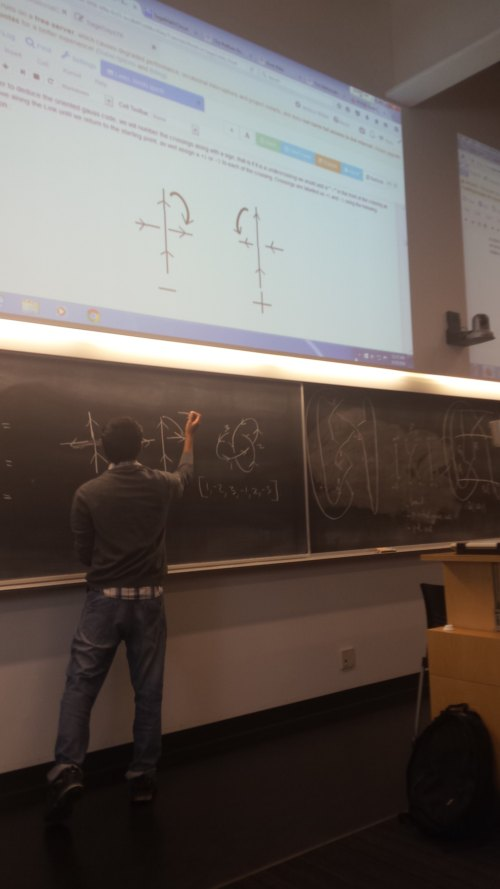
\includegraphics[scale=0.3]{pictures/sd78-1.jpg}
&
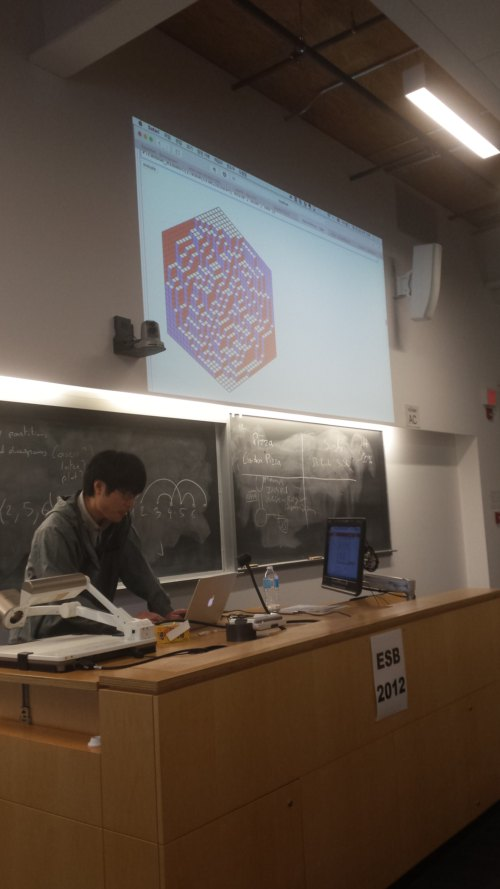
\includegraphics[scale=0.3]{pictures/sd78-2.jpg}
\end{tabular}
\end{figure}



\end{event}
